% Do NOT change this "Section" title
% and do NOT add more "Section" level titles.
\section{Implementation}\label{sec:implementation}
Overview of the motor and motor controller system:
\begin{figure}[h]
    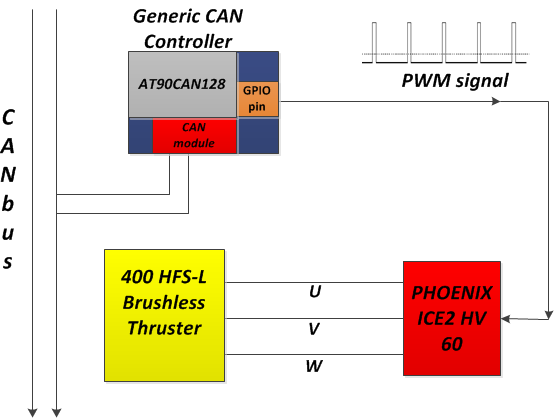
\includegraphics[width=0.5\textwidth]{./figure/figA.png}
    \caption{Motor and motor controller system overview}
    \label{fig:one_column_figure}
\end{figure}

The implementation has the following parts:
\begin{itemize}
\item Thrusters
\item Thruster speed controller
 \item CAN message processing
 \item Generating the PWM signal
 \item Main program 
\end{itemize}

% You can use how many "subsections" and "subsubsections" you like.
\subsection{Thrusters}
During the selection of thrusters only two models seemed to satisfy the needs of the "Naiad". One was the SeaBotix BTD150 which is a brushed DC thruster very popular, and the other one was the CrustCrawler 400HFSL brushless DC thruster which is not as popular as the first one and a little more expensive. After the advantages and disadvantages were considered the CrustCrawler 400HFS-L has been decided to be the better option for Naiad by being lighter, more power efficient and more powerfull than the SeaBotix BTD150. 

\begin{table}[h]
\centering
    \caption{CrustCrwler 400 HFS-L specifications}
    \begin{tabular}{|c|c|} \hline
    \label{table:one_column}
       Motor type    &  High efficiency brushless \\ \hline
       Weight(motor) & 185 g \\ \hline
         Weight(thruster) & 255 g \\ \hline
           Max power &  130 W \\ \hline
             Gear ratio & 4.28:1 \\ \hline
               Operating voltage & 12 to 50 Volts \\ \hline
                 Depth rating  & 300 ft. \\ \hline
                   Thruster Housing & T-6 Aluminum \\ \hline
                     Thruster length & 15.87 cm \\ \hline  
                      Propeller size & 60 mm \\ \hline
     
    \end{tabular}
\end{table}
 
\subsection{Thrusters speed controller}
The CrustCrawler 400 HFS-L's brushless motor has three winding U, V and W and cannot be connected directly to the Generic CAN controller that has no feature to control brushless motors. So a special speed controller had to be used to in order to actuate the thrusters. After a research and comparison of different brushless controllers a decision has been made to go for the one suggested by the thruster manufacturer and that is the Phoenix ICE2 HV 60 thruster controller. A feature of this brushless controller is that it has a learning function so that you can calibrate the controller for use in different systems. 

The principle of operation of the controller is to take as input a PWM signal and to convert it in signals for the three winding brushless motor. The input can be calibrated with the learning function by holding for  a few seconds the throttle in the maximum position then in the minimum position and then in the middle position. Always the position of the throttle at the power up of the controller has to be the middle one. Keeping it in the maximum position at start up will cause the controller to go into the configuration mode. By moving the throttle to different values the output will change and will cause the thruster to increase its speed or decrease it depending on what action has been taken. 
\subsection{CAN message processing}
The speed of the thrusters will be adjusted several times a second. This is done by receiving from the CAN bus messages that contain the actuation value. The received CAN message consists of six bytes out of maximum of 8 specified in the CAN bus. 

Each of the bytes will represent an actuation value for a thruster so for example the CAN message is received by all the thrusters but each of the thrusters will use only one byte from the message. The thruster with id 1 will use the first byte, the thruster with id 2 will use the value from the second byte and so on. Each byte contains a 8 bit signed value but the structure in which the CAN message is saved when it is received is 8 bytes of unsigned values. So for the correct interpretation of the data a conversion has to be made using Ada Unchecked conversion feature of Ada programming language which copies the bits from one type of variable and writes them in another type of variable without raising any exceptions if the sizes of the two type are equal or the empty one is bigger.  
\subsection{Generating the PWM signal}
The PWM signal is used to control the speed of the thrusters and also the direction of the thrust (forward or backward). The PWM signal is created by the Generic CAN controller and then fed to the brushless speed controller. The brushless speed controller expects a PWM signal with the pulse width of 1 to 2 ms every 6 to 25 ms. This PWM signal is created by configuring some registers of the AT90CAN128 MCU.

 The period of the pulse is configured with the ICR1 register and set to 16.3 ms with a resolution of 4096. To generate the pulse another register is used: OCR1A which at each Timer1 increment is compared with TCNT1 register which keeps track of current number of clock ticks and if they match the value on the output pin is set to 0 and the TCNT1 register is set back to 0. 

\subsection{Main program}
The main program consists of a loop in which the CAN message processing and the generation of the PWM signal is done. Inside the endless loop the function that reads the CAN messages from the buffer is called and if there are any available CAN messages in the buffer they will be processed or if not it will wait for the specified amount of time for a message to be received and then skip to the next instruction.

 